\appendices

\section{Existence of harmful risk-prone clients}
\label{app:harmful_risk_prone_client}
Let $S\subseteq\mathcal{C}$ be a currently retained client-block set and let 
$j\in\mathcal{C}\setminus S$ be an additional candidate client. 
Denote $S^+=S\cup\{j\}$. 
Suppose the target-risk upper bound for subset $S$ is written as
\[
\mathcal{B}(S)
=
\epsilon_S^n(h_S)
+
\xi_{\mathrm{noise}}(S)
+
\mathcal{D}(T||S).
\]
Define the data-benefit term of adding client $j$ as
\[
G_j(S)
=
\epsilon_S^n(h_S)
-
\epsilon_{S^+}^n(h_{S^+}),
\]
and define the risk-increase term as
\[
R_j(S)
=
\left[
\xi_{\mathrm{noise}}(S^+)-\xi_{\mathrm{noise}}(S)
\right]
+
\left[\mathcal{D}(T||S^+)
-
\mathcal{D}(T||S)\right].
\]
If
\[
R_j(S)>G_j(S),
\]
then
\[
\mathcal{B}(S^+)>\mathcal{B}(S).
\]
That is, retaining client $j$ worsens the target-risk upper bound, which justifies removing such risk-prone client blocks before training.


\begin{proof}
By definition,
\[
\begin{aligned}
\mathcal{B}(S^+)-\mathcal{B}(S)
&=
\epsilon_{S^+}^n(h_{S^+})
-
\epsilon_S^n(h_S)
\\
&\quad+
\left[
\xi_{\mathrm{noise}}(S^+)-\xi_{\mathrm{noise}}(S)
\right]
\\
&\quad+
\left[\mathcal{D}(T||S^+)
-
\mathcal{D}(T||S)\right].
\\
&=
-G_j(S)+R_j(S).
\end{aligned}
\]
Therefore, if $R_j(S)>G_j(S)$, then 
$\mathcal{B}(S^+)-\mathcal{B}(S)>0$, which proves the claim.
\end{proof}

\section{Additional theoretical details}
\label{app:theory_appendix}
\subsection{Proof of Lemma~\ref{lem:noise_bridge}}
\begin{proof}
For any distribution $P$ over $(X,Y)$, the risk of $h$ is defined as
$\epsilon_P(h)=\mathbb E_{(X,Y)\sim P}[\ell(h(X),Y)]$.
Since $\mathcal Y=\{1,\dots,K\}$ is discrete, by the law of total expectation,
\begin{align}
\epsilon_P(h)
&=
\mathbb E_{X}
\left[
\mathbb E_{Y\mid X}
\left[
\ell(h(X),Y)
\mid X
\right]
\right] \\
&=
\mathbb E_{x\sim P_X}
\left[
\sum_{c=1}^{K}
P(Y=c\mid x)\ell(h(x),c)
\right].
\label{eq:risk_total_expectation}
\end{align}
Under Assumption~\ref{assump:label_only_noise}, $P_S^c(X,Y)$ and $P_S^n(X,\widetilde Y)$ share the same input marginal $P_S^X$.
Applying Eq.~\eqref{eq:risk_total_expectation} to the clean and noisy mixtures gives
\begin{align}
\epsilon_S^c(h)
&=
\mathbb{E}_{x\sim P_S^X}
\left[
\sum_{c=1}^{K}
P_S^c(Y=c\mid x)
\ell(h(x),c)
\right],\\
\epsilon_S^n(h)
&=
\mathbb{E}_{x\sim P_S^X}
\left[
\sum_{c=1}^{K}
P_S^n(\widetilde Y=c\mid x)
\ell(h(x),c)
\right].
\end{align}
Therefore,
\begin{align}
&\big|\epsilon_S^c(h)-\epsilon_S^n(h)\big|\\
&= \Bigg|
\mathbb{E}_{x\sim P_S^X} \sum_{c=1}^{K} 
\Big( P_S^c(Y=c\mid x) - P_S^n(\widetilde Y=c\mid x) \Big)
\ell(h(x),c)
\Bigg| \notag \\
&\le \mathbb{E}_{x\sim P_S^X} 
\sum_{c=1}^{K} 
\Big| P_S^c(Y=c\mid x) - P_S^n(\widetilde Y=c\mid x) \Big|
\cdot |\ell(h(x),c)| \notag \\
&\le \mathbb{E}_{x\sim P_S^X} 
\sum_{c=1}^{K} 
\Big| P_S^c(Y=c\mid x) - P_S^n(\widetilde Y=c\mid x) \Big| \notag \\
&= \xi_{\mathrm{noise}}(S)
\end{align}
The first inequality follows from the triangle inequality, and the second follows from the bounded-loss assumption $0\le \ell\le 1$.
\end{proof}

\subsection{Proof of Lemma~\ref{lem:label_shift_transfer}}
\begin{proof}
By the standard variational characterization of total variation distance~\cite{gibbs2002choosing}, for any measurable function $f$ with $0\le f\le 1$,
\[
\left|
\mathbb E_P[f]-\mathbb E_Q[f]
\right|
\le
\mathrm{TV}(P,Q).
\]
Applying this inequality to $f_h(x,y)=\ell(h(x),y)$ yields
\begin{align}
&\big|\epsilon_T(h)-\epsilon_S^c(h)\big| \\
&=
\left|
\mathbb{E}_{(x,y)\sim P_T}
\left[
\ell(h(x),y)
\right]
-
\mathbb{E}_{(x,y)\sim P_S^c}
\left[
\ell(h(x),y)
\right]
\right| \\
&\le
\mathrm{TV}(P_T,P_S^c).
\end{align}
Since the class-conditional distributions are shared,
\begin{equation}
\label{eq:TV_equality}
\mathrm{TV}(P_T,P_S^c)
=
\frac{1}{2}
\sum_{y=1}^{K}
\left|
q_T(y)-\bar q_S(y)
\right|
=
\frac{1}{2}
\|\bar q_S-q_T\|_1.
\end{equation}
Therefore,
\[
\epsilon_T(h)
\le
\epsilon_S^c(h)
+
\frac{1}{2}\|\bar q_S-q_T\|_1.
\]
\end{proof}
\subsection{Proof of Theorem~\ref{thm:residualized_probing_bound}}
\begin{proof}
By Theorem~\ref{thm:main_bound},
\begin{equation}
\epsilon_T(h)
\le
\epsilon_S^n(h)
+
\xi_{\mathrm{noise}}(S)
+
\frac12\|\bar q_S-q_T\|_1.
\end{equation}
By the definition of $r_H(S;c_H)$, we have
\begin{equation}
\xi_{\mathrm{noise}}(S)
\le
c_H\widehat{\xi}_{H}(S)
+
r_H(S;c_H).
\end{equation}
For the distribution mismatch term, the triangle inequality gives
\begin{align}
\frac12\|\bar q_S-q_T\|_1
&\le
\frac12\|\bar q_S-z_S\|_1
+
\frac12\|z_S-z_S^\epsilon\|_1
\\&+
\frac12\|z_S^\epsilon-p_{\mathrm{prob}}\|_1
+
\frac12\|p_{\mathrm{prob}}-q_T\|_1\\
&=
r_Z(S)
+
r_\epsilon(S)
+
\mathrm{TV}(z_S^\epsilon,p_{\mathrm{prob}})
+
r_T.
\end{align}
By Pinsker's inequality, also known as the Csisz{\'a}r--Kullback--Pinsker inequality~\cite{pinsker1964information,csiszar1967information},
\begin{equation}
\mathrm{TV}(z_S^\epsilon,p_{\mathrm{prob}})
\le
\sqrt{
\frac12
\mathrm{KL}
\left(
p_{\mathrm{prob}}\|z_S^\epsilon
\right)
}.
\end{equation}
Combining the above inequalities gives Eq.~\eqref{eq:residualized_probing_bound}.
\end{proof}
\subsection{Proof of Corollary~\ref{cor:probing_consistency_surrogate}}
\begin{proof}
By Theorem~\ref{thm:residualized_probing_bound},
\begin{align}
\epsilon_T(h)
&\le
\epsilon_S^n(h)
+
c_H\widehat{\xi}_{H}(S) \\
&
+
\sqrt{
\frac12
\mathrm{KL}
\left(
p_{\mathrm{prob}}\|z_S^\epsilon
\right)
}
+
R_{\mathrm{prob}}(S;c_H).
\end{align}
For any $x\ge0$ and $\lambda_s>0$, Young's inequality gives
$\sqrt{x/2}\le \lambda_s x + 1/(8\lambda_s)$.
Applying this inequality to $x=\mathrm{KL}(p_{\mathrm{prob}}\|z_S^\epsilon)$ and using
$R_{\mathrm{prob}}(S;c_H)\le\delta_{\mathrm{prob}}$ gives Eq.~\eqref{eq:probing_consistency_bound}.
\end{proof}
\subsection{Derivation of the Label-Prior TV Distance}
\label{app:tv_label_prior}

This appendix proves that, under the shared class-conditional assumption, the total variation distance between the target distribution and the selected clean client mixture reduces to the $\ell_1$ distance between their label priors.

Recall Assumption~\ref{assump:label_shift}. 
The target distribution and the selected clean client mixture are written as
\[
P_T(x,y)=p(x\mid y)q_T(y),
\qquad
P_S^c(x,y)=p(x\mid y)\bar q_S(y),
\]
where
\[
\bar q_S=\sum_{i\in S}w_i(S)q_i.
\]
Using the definition of total variation distance,
\begin{align}
&\mathrm{TV}(P_T,P_S^c)\\
&=
\frac{1}{2}
\sum_{y=1}^{K}
\int
\left|
P_T(x,y)-P_S^c(x,y)
\right|
dx \\
&=
\frac{1}{2}
\sum_{y=1}^{K}
\int
\left|
p(x\mid y)q_T(y)
-
p(x\mid y)\bar q_S(y)
\right|
dx \\
&=
\frac{1}{2}
\sum_{y=1}^{K}
\int
p(x\mid y)
\left|
q_T(y)-\bar q_S(y)
\right|
dx \\
&=
\frac{1}{2}
\sum_{y=1}^{K}
\left|
q_T(y)-\bar q_S(y)
\right|
\int p(x\mid y)dx.
\end{align}
Since $p(x\mid y)$ is a conditional distribution, $\int p(x\mid y)dx=1$ for every class $y$. 
Therefore,
\begin{equation}
\mathrm{TV}(P_T,P_S^c)
=
\frac{1}{2}
\sum_{y=1}^{K}
\left|
q_T(y)-\bar q_S(y)
\right|
=
\frac{1}{2}
\|\bar q_S-q_T\|_1.
\end{equation}

Thus, under shared class-conditional distributions, the source--target discrepancy is fully determined by the mismatch between the selected client label prior $\bar q_S$ and the target label prior $q_T$.

\subsection{Entropy as a probing for client noise}
\label{app:entropy_probing}

We now formalize why average predictive entropy is a useful reliability signal.

\begin{proposition}[Entropy--noise bridge]
\label{prop:entropy_bridge_appendix}
Fix client $i$ and assume $K$-class symmetric label noise with rate $\rho_i\in[0,1-1/K)$. Let
\begin{equation}
T_{\rho_i}
=
(1-\rho_i)I + \frac{\rho_i}{K-1}(\mathbf{1}\mathbf{1}^\top-I)
\end{equation}
be the noise transition matrix. For a probing input $x$, denote the clean posterior by $\eta_i(x)\in\Delta^{K-1}$ and the noisy posterior by
\begin{equation}
\tilde \eta_i(x)=T_{\rho_i}\eta_i(x).
\end{equation}
Assume the probing samples are $\delta_{\mathrm{sep}}$-separable in the sense that
\begin{equation}
\max_c \eta_i(c\mid x) \ge 1-\delta_{\mathrm{sep}},
\qquad \forall x\in\mathcal{D}_{\mathrm{prob}},
\end{equation}
for some $\delta_{\mathrm{sep}}\in[0,1)$. Assume further that the local model predictions satisfy
\begin{equation}
\mathbb{E}_{x\sim P_{\mathrm{prob}}}
\big[
\mathrm{KL}(\tilde\eta_i(x)\,\|\,p_i(\cdot\mid x))
\big]
\le \varepsilon_{\mathrm{cal}}.
\end{equation}
Define
\begin{equation}
 h_K(\rho)
 :=
 -(1-\rho)\log(1-\rho)
 - \rho\log\frac{\rho}{K-1}.
\end{equation}
Then the average predictive entropy
\begin{equation}
\bar H_i
:=
\mathbb{E}_{x\sim P_{\mathrm{prob}}}
\big[H(p_i(\cdot\mid x))\big]
\end{equation}
obeys
\begin{equation}
\label{eq:entropy_bridge_appendix}
\bar H_i
\ge
(1-\delta_{\mathrm{sep}})h_K(\rho_i)
- \phi_K\!\left(\sqrt{\varepsilon_{\mathrm{cal}}/2}\right),
\end{equation}
where
\begin{align}
\phi_K(\delta)
&:=\delta\log(K-1)+h_2(\delta),\\
h_2(\delta)
&:=-\delta\log\delta-(1-\delta)\log(1-\delta).
\end{align}
Consequently, $\bar H_i$ is monotone increasing in $\rho_i$ up to a calibration- and separability-dependent relaxation.
\end{proposition}

\begin{proof}
Fix a probing point $x$ and let $c^*(x):=\arg\max_c \eta_i(c\mid x)$. By separability, there exists a distribution $r_x\in\Delta^{K-1}$ such that
\begin{equation}
\eta_i(x)
=
(1-\delta_x)e_{c^*(x)} + \delta_x r_x,
\qquad 0\le \delta_x \le \delta_{\mathrm{sep}}.
\end{equation}
Applying the symmetric transition matrix gives
\begin{equation}
\tilde\eta_i(x)
=
(1-\delta_x)v_{\rho_i,c^*(x)} + \delta_x T_{\rho_i}r_x,
\end{equation}
where
\begin{equation}
v_{\rho_i,c^*}
:=
(1-\rho_i)e_{c^*}
+ \frac{\rho_i}{K-1}(\mathbf{1}-e_{c^*}).
\end{equation}
By concavity of entropy,
\begin{align}
H(\tilde\eta_i(x))
&\ge
(1-\delta_x)H\big(v_{\rho_i,c^*(x)}\big)
+\delta_x H\big(T_{\rho_i}r_x\big) \\
&\ge
(1-\delta_x)h_K(\rho_i)
\ge
(1-\delta_{\mathrm{sep}})h_K(\rho_i).
\end{align}
Now compare $p_i(\cdot\mid x)$ and $\tilde\eta_i(x)$. By Pinsker's inequality,
\begin{equation}
\|p_i(\cdot\mid x)-\tilde\eta_i(x)\|_1
\le
\sqrt{2\,\mathrm{KL}(\tilde\eta_i(x)\,\|\,p_i(\cdot\mid x))}.
\end{equation}
The Fannes--Audenaert continuity bound for entropy implies~\cite{audenaert2007sharp}
\begin{equation}
\big|H(p_i(\cdot\mid x))-H(\tilde\eta_i(x))\big|
\le
\phi_K\!\left(\tfrac{1}{2}\|p_i(\cdot\mid x)-\tilde\eta_i(x)\|_1\right).
\end{equation}
Using Pinsker and Jensen,
\begin{equation}
\mathbb{E}_{x}\big[H(p_i(\cdot\mid x))\big]
\ge
\mathbb{E}_{x}\big[H(\tilde\eta_i(x))\big]
-
\phi_K\!\left(\sqrt{\varepsilon_{\mathrm{cal}}/2}\right).
\end{equation}
Combining with the lower bound on $H(\tilde\eta_i(x))$ yields \eqref{eq:entropy_bridge_appendix}. Finally, $h_K(\rho)$ is strictly increasing on $[0,1-1/K)$, so the ranking induced by $\bar H_i$ agrees with the ranking induced by $\rho_i$ up to the stated relaxation. \qed
\end{proof}

\paragraph{\textbf{A useful corollary.}}
Since $h_K$ is invertible on $[0,1-1/K)$, \eqref{eq:entropy_bridge_appendix} implies the conservative upper bound
\begin{equation}
\rho_i
\le
h_K^{-1}\!\left(
\frac{\bar H_i+\phi_K(\sqrt{\varepsilon_{\mathrm{cal}}/2})}{1-\delta_{\mathrm{sep}}}
\right).
\end{equation}
Under symmetric noise, this immediately yields
\begin{equation}
\xi_{\mathrm{noise}}(S)
\lesssim
2\sum_{i\in S}w_i(S)
\,h_K^{-1}\!\left(
\frac{\bar H_i+\phi_K(\sqrt{\varepsilon_{\mathrm{cal}}/2})}{1-\delta_{\mathrm{sep}}}
\right),
\end{equation}
which motivates the reliability score used in the main text.

\subsection{Combinatorial optimization and a submodular variant}
\label{app:submodular_variant}

The main algorithm uses a KL-based target-matching objective because it directly aligns the retained subset with the probing target distribution. This objective is not guaranteed to be submodular. Nevertheless, the connection to classical subset selection can be made explicit via a closely related facility-location surrogate~\cite{nemhauser1978submodular,krause2014submodular,sener2018coreset,mirzasoleiman2020coresets_dataefficient_pmlr}.

Let $\kappa(i,j)\ge 0$ be a similarity between the predictive signatures $z_i$ and $z_j$ defined in the main text. Consider the coverage function
\begin{equation}
G(S) := \sum_{j=1}^N \max_{i\in S} \kappa(i,j),
\end{equation}
and the set objective
\begin{equation}
F_{\mathrm{sub}}(S)
:=
\lambda_r\sum_{i\in S} r_i
+ \lambda_s G(S),
\qquad \lambda_r,\lambda_s\ge 0.
\end{equation}
The first term rewards reliable clients; the second term rewards representative coverage of the predictive-signature space.

\begin{proposition}[Submodular subset view]
\label{prop:submodular_appendix}
$F_{\mathrm{sub}}$ is monotone submodular. Consequently, maximizing $F_{\mathrm{sub}}(S)$ subject to $|S|\le M$ is NP-hard in general, and the classical greedy algorithm returns a subset $S_{\mathrm{greedy}}$ satisfying
\begin{equation}
F_{\mathrm{sub}}(S_{\mathrm{greedy}})
\ge
\left(1-\frac{1}{e}\right)
\max_{|S|\le M}F_{\mathrm{sub}}(S)
\end{equation}
\cite{nemhauser1978submodular,krause2014submodular}.
\end{proposition}

\begin{proof}
The modular term $\sum_{i\in S}r_i$ is monotone submodular because its marginal gain is constant. The facility-location term $G(S)$ is also monotone submodular: adding an element can only increase the pointwise maxima, and the marginal gain decreases as the current subset grows. A nonnegative linear combination of monotone submodular functions remains monotone submodular. The $(1-1/e)$ guarantee then follows from the classical theorem of Nemhauser \emph{et al.} \cite{nemhauser1978submodular}. \qed
\end{proof}

\paragraph{\textbf{Interpretation.}}
This proposition clarifies the conceptual role of FedOCR. The retained participant pool can be viewed as an \emph{outlier-removal client set}: it compresses the candidate population into a smaller block-level subset that preserves representative coverage while filtering out unreliable or outlying clients.

\section{Discussion on probing-Consistency Residuals}
\label{app:probing_consistency}

This appendix discusses when the residual terms in the residualized probing outlier-removal bound are expected to be small.
Recall that Theorem~\ref{thm:residualized_probing_bound} separates the observable probing objective from the approximation residual
\[
R_{\mathrm{prob}}(S;c_H)
=
r_H(S;c_H)
+
r_Z(S)
+
r_T
+
r_\epsilon(S),
\]
where
\[
\begin{aligned}
r_H(S;c_H)
&=
\left[
\xi_{\mathrm{noise}}(S)
-
c_H\widehat{\xi}_{H}(S)
\right]_+,
\\
r_Z(S)
&=
\frac12\|\bar q_S-z_S\|_1,
\\
r_T
&=
\frac12\|p_{\mathrm{prob}}-q_T\|_1,
\\
r_\epsilon(S)
&=
\frac12\|z_S-z_S^\epsilon\|_1.
\end{aligned}
\]
These residuals are not directly optimized by FedOCR.
They quantify the gap between the population quantities in Theorem~\ref{thm:main_bound} and the probing statistics used by the algorithm.
The probing bound should therefore be interpreted conditionally: when these residuals are small, optimizing the observable entropy--KL surrogate is aligned with reducing the target-risk upper bound.

\subsection{When is the entropy residual $r_H$ small?}
\label{app:entropy_residual}

The entropy residual
\[
r_H(S;c_H)
=
\left[
\xi_{\mathrm{noise}}(S)
-
c_H\widehat{\xi}_{H}(S)
\right]_+
\]
measures whether the entropy-based probing underestimates the population label-noise discrepancy.
It is small when probing predictive entropy is positively aligned with client-level predictive unreliability induced by corrupted supervision.

This condition is more plausible when the following factors hold.
First, the probing set should be representative of the target decision regions, so that uncertainty on $\mathcal D_{\mathrm{prob}}$ reflects the instability of a locally adapted client model on target-relevant inputs.
Second, the local adaptation step should be long enough for the client model $f_i$ to reflect the statistical quality of client $i$, but not so long that it overfits corrupted labels with overconfident predictions.
Third, the model should be reasonably calibrated on the probing distribution, so that predictive entropy is meaningful as an uncertainty measure~\cite{guo2017calibration}.
Under these conditions, clients with stronger label corruption tend to produce less stable or less confident predictions on the probing set, leading to larger $\widetilde H_i$.

However, predictive entropy is not a noise-specific statistic.
A large entropy value can also arise from hard examples, feature shift, model underfitting, class imbalance, or probing-client mismatch.
Conversely, a heavily corrupted client may become overconfident after local overfitting, producing low entropy despite poor label quality.
For this reason, FedOCR interprets entropy as a probing-set predictive unreliability measure rather than a direct estimator of the true label-noise rate.
In our experiments, we empirically examine the relationship between client noise severity and probing predictive entropy to support this probing choice.

\subsection{When is the coverage residual $r_Z$ small?}
\label{app:coverage_residual}

The coverage residual
\[
r_Z(S)
=
\frac12\|\bar q_S-z_S\|_1
\]
measures the mismatch between the clean selected-client label prior $\bar q_S$ and the probing-predicted mixture $z_S$.
This residual is small when the probing-predicted signatures preserve the relative target-facing class coverage of the retained clients, echoing the importance of source--target distribution alignment in domain adaptation and Non-IID FL~\cite{ben2010theory,hsu2019measuring,zhu2021survey}.

This condition does not require $z_S$ to exactly recover each client's private clean label prior.
Instead, it requires that the probing predictions of the locally adapted client models provide a useful class-profile signal for how the retained client pool behaves on target-relevant inputs.
The condition is more plausible when the probing set covers the target classes, the adapted client models retain class-discriminative information from their local data, and the hard prediction signatures are not dominated by noise or underfitting.
The sample-size weighting in $z_S=\sum_{i\in S}\omega_i(S)\hat r_i$ also mirrors the mixture prior $\bar q_S=\sum_{i\in S}w_i(S)q_i$, which helps align the probing mixture with the population mixture when the signatures are informative.

The residual can be large when client models are poorly adapted, when local label noise severely distorts decision boundaries, or when the probing distribution is far from the regions where client models are informative.
It can also be large under strong feature shift, because a client may have a useful local class distribution but produce biased predictions on the probing set.
Therefore, $z_S$ should be understood as a target-facing predictive coverage statistic rather than an exact estimator of private clean label priors.

\subsection{When is the target-prior residual $r_T$ small?}
\label{app:target_prior_residual}

The target-prior residual
\[
r_T
=
\frac12\|p_{\mathrm{prob}}-q_T\|_1
\]
measures how well the server-side reference prior approximates the target label prior.
It is small when this reference prior is specified to match the target task~\cite{ben2010theory,lipton2018labelshift}.
For example, in a balanced classification benchmark, a uniform reference prior yields a small $r_T$ when the target prior is also balanced.
This does not require using the true labels of the probing samples.
In practical deployments, this residual can be reduced by choosing the reference prior according to the expected deployment distribution.

This residual can be large if the reference prior is biased, outdated, or mismatched with the target population.
In that case, the KL term $\mathrm{KL}(p_{\mathrm{prob}}\|z_S^\epsilon)$ encourages matching the reference prior rather than the true target prior.
Thus, the reliability of the representativeness surrogate depends on both the reference prior and the probing input distribution.

\subsection{Effect of the smoothing residual $r_\epsilon$}
\label{app:smoothing_residual}

The smoothing residual
\[
r_\epsilon(S)
=
\frac12\|z_S-z_S^\epsilon\|_1
\]
is introduced only for numerical stability when computing the forward KL divergence.
Since
\[
z_S^\epsilon(c)
=
\frac{z_S(c)+\epsilon}{1+K\epsilon},
\qquad c=1,\dots,K,
\]
we have $z_S^\epsilon(c)>0$ for every class, which avoids zero-support problems in $\mathrm{KL}(p_{\mathrm{prob}}\|z_S^\epsilon)$.
For small $\epsilon$, the perturbation from $z_S$ to $z_S^\epsilon$ is small.
Indeed,
\[
z_S^\epsilon-z_S
=
\frac{\epsilon\mathbf 1-K\epsilon z_S}{1+K\epsilon},
\]
and therefore
\[
\|z_S^\epsilon-z_S\|_1
\le
\frac{\epsilon\|\mathbf 1\|_1+K\epsilon\|z_S\|_1}{1+K\epsilon}
=
\frac{2K\epsilon}{1+K\epsilon}.
\]
Thus,
\[
r_\epsilon(S)
=
\frac12\|z_S-z_S^\epsilon\|_1
\le
\frac{K\epsilon}{1+K\epsilon}.
\]
When $\epsilon$ is small, this residual is negligible compared with the main probing terms.

\subsection{Summary}
\label{app:probing_consistency_summary}

The residualized bound separates two roles.
The observable part,
\[
c_H\widehat{\xi}_{H}(S)
+
\lambda_s\mathrm{KL}(p_{\mathrm{prob}}\|z_S^\epsilon),
\]
is the quantity optimized by FedOCR.
The residual part,
\[
R_{\mathrm{prob}}(S;c_H)
=
r_H(S;c_H)+r_Z(S)+r_T+r_\epsilon(S),
\]
measures how well the probing statistics approximate the corresponding population quantities.
Therefore, the theoretical role of FedOCR is conditional rather than unconditional: if the probing set is target-relevant and the adapted client models yield informative uncertainty and class-signature statistics, then minimizing the entropy--KL surrogate is aligned with reducing the target-risk upper bound.

\section{Oracle Experiment Details}
\label{app:oracle_experiment_details}
This appendix records the controlled oracle validation that is summarized briefly in the main text.
We consider a three-class Gaussian classification problem with two-dimensional features, class-balanced target prior, and six candidate clients that differ in both label prior and symmetric label-noise rate.
The purpose of this experiment is not to benchmark practical methods, but to check whether the risk factors in Theorem~\ref{thm:main_bound} rank retained client-block sets in the expected order.
The four retention strategies isolate the effects of no outlier removal, distribution mismatch, label noise, and the oracle FedOCR-style admission rule.
\begin{table}[t]
\centering
\caption{\normalfont Configuration of the oracle experiment. The six clients differ in both class-prior distribution and label-noise rate. Clients C1--C3 are low-noise but individually class-skewed, while their union provides a balanced class distribution.}
\label{tab:oracle_setup_appendix}
\setlength{\tabcolsep}{4pt}
\renewcommand{\arraystretch}{1.15}
\begin{tabular}{l|l}
\toprule
\textbf{Item} & \textbf{Setting} \\
\midrule
Task type & Three-class non-IID classification \\
Feature dimension & 2 \\
Input distribution & Gaussian class-conditionals \\
Class means & $\mu_1=(-2,0),\ \mu_2=(2,0),\ \mu_3=(0,2)$ \\
Covariance & $\sigma=0.9$ \\
Target prior & $q_T=(1/3,1/3,1/3)$ \\
Label noise & Symmetric noise with rate $\rho$ \\
Noise mechanism & Flip to other $K-1$ classes uniformly \\
Model & Two-layer MLP, $2 \rightarrow 16 \rightarrow 3$ \\
Activation & ReLU \\
Optimizer & Full-batch gradient descent \\
Learning rate & $0.01$ \\
Training epochs & 400 epochs, including epoch 0 initialization \\
Initialization & $\mathcal{N}(0,0.01)$ with fixed random seed \\
Samples per client & 300 \\
Target test set & 3000 clean samples with balanced class prior \\
\bottomrule
\end{tabular}
\end{table}

\paragraph{\textbf{Oracle results.}}
The oracle bound and target-risk figures below show the same qualitative pattern described in the main text.
The FedOCR ideal subset achieves the lowest theoretical bound because it reduces both the label-noise term and the distribution-mismatch term, while the balanced noisy subset has the largest bound.
The empirical target-risk curves further confirm that the FedOCR ideal subset attains the lowest target risk and the smallest bound gap.

\section{Experimental Setup Details}
\label{app:experiment_setup_details}
\subsection{Main experiment setup}
\label{app:main_experiment_setup}
We evaluate on MedMNIST~\cite{yang2023medmnist} and CIFAR-10/100~\cite{krizhevsky2009learning}.
Unless otherwise specified, the training data are split over $N=50$ clients and $K=20$ clients participate in each federated training run.
We use Dirichlet partitioning with concentration parameter $\alpha=0.5$ and a step-imbalance ratio of 5 to simulate Non-IID data~\cite{hsu2019measuring,li2021silos,zhu2021survey}.
Label noise is applied symmetrically at the client level, following standard noisy-label robustness protocols~\cite{natarajan2013learning,patrini2017loss,liang2023fednoisy}.
The main experiments use linear and Gaussian heterogeneous noise.
All methods are trained for $T=200$ global rounds under the same maximum round budget.
For FedOCR's admission stage, we use a short 10-epoch local adaptation to compute the filtering indicators, which keeps the pre-screening lightweight and consistent with the deployment-oriented design.
For local training, we use Adam with learning rate $1\times10^{-4}$ and batch size 64.



\section{Supplementary Experimental Curves}
\label{app:more_curves}

To avoid excessive repetition in the main text, we present only the CIFAR-10 result under linear heterogeneous noise as the main illustration. This appendix further provides the complete convergence curves for the remaining settings under the same diagnostic setup, in order to supplement the evidence for the general effectiveness of FedOCR.
Across the appendix benchmarks, the main pattern is consistent: FedOCR achieves higher final accuracy and more stable convergence when the same client-block outlier-removal rule is applied under heterogeneous client-level label noise.
The linear setting is especially diagnostic because it exposes the method to a wide range of client noise rates within the same federation.
\begin{figure*}[t]
    \centering
    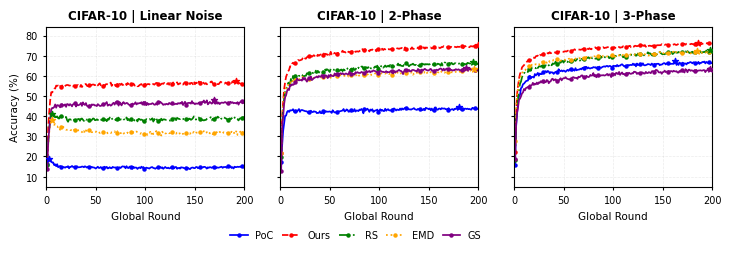
\includegraphics[width=\textwidth]{figure/appendix_compare_cifar10.png}
    \caption{Test accuracy curves under linear heterogeneous noise in the appendix benchmark suite. FedOCR achieves higher final accuracy and more stable convergence than the compared baselines.}
    \label{fig:triple_figures}
\end{figure*}

\begin{figure*}[t]
    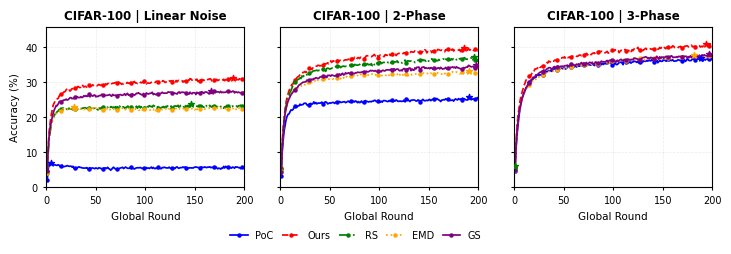
\includegraphics[width=\textwidth]{figure/appendix_compare_cifar100.png}
    \caption{Additional convergence curves on CIFAR-100 under linear heterogeneous real-imitation noise.}
    \label{fig:appendix_cifar100}
\end{figure*}

\begin{figure}[h]
    \centering
    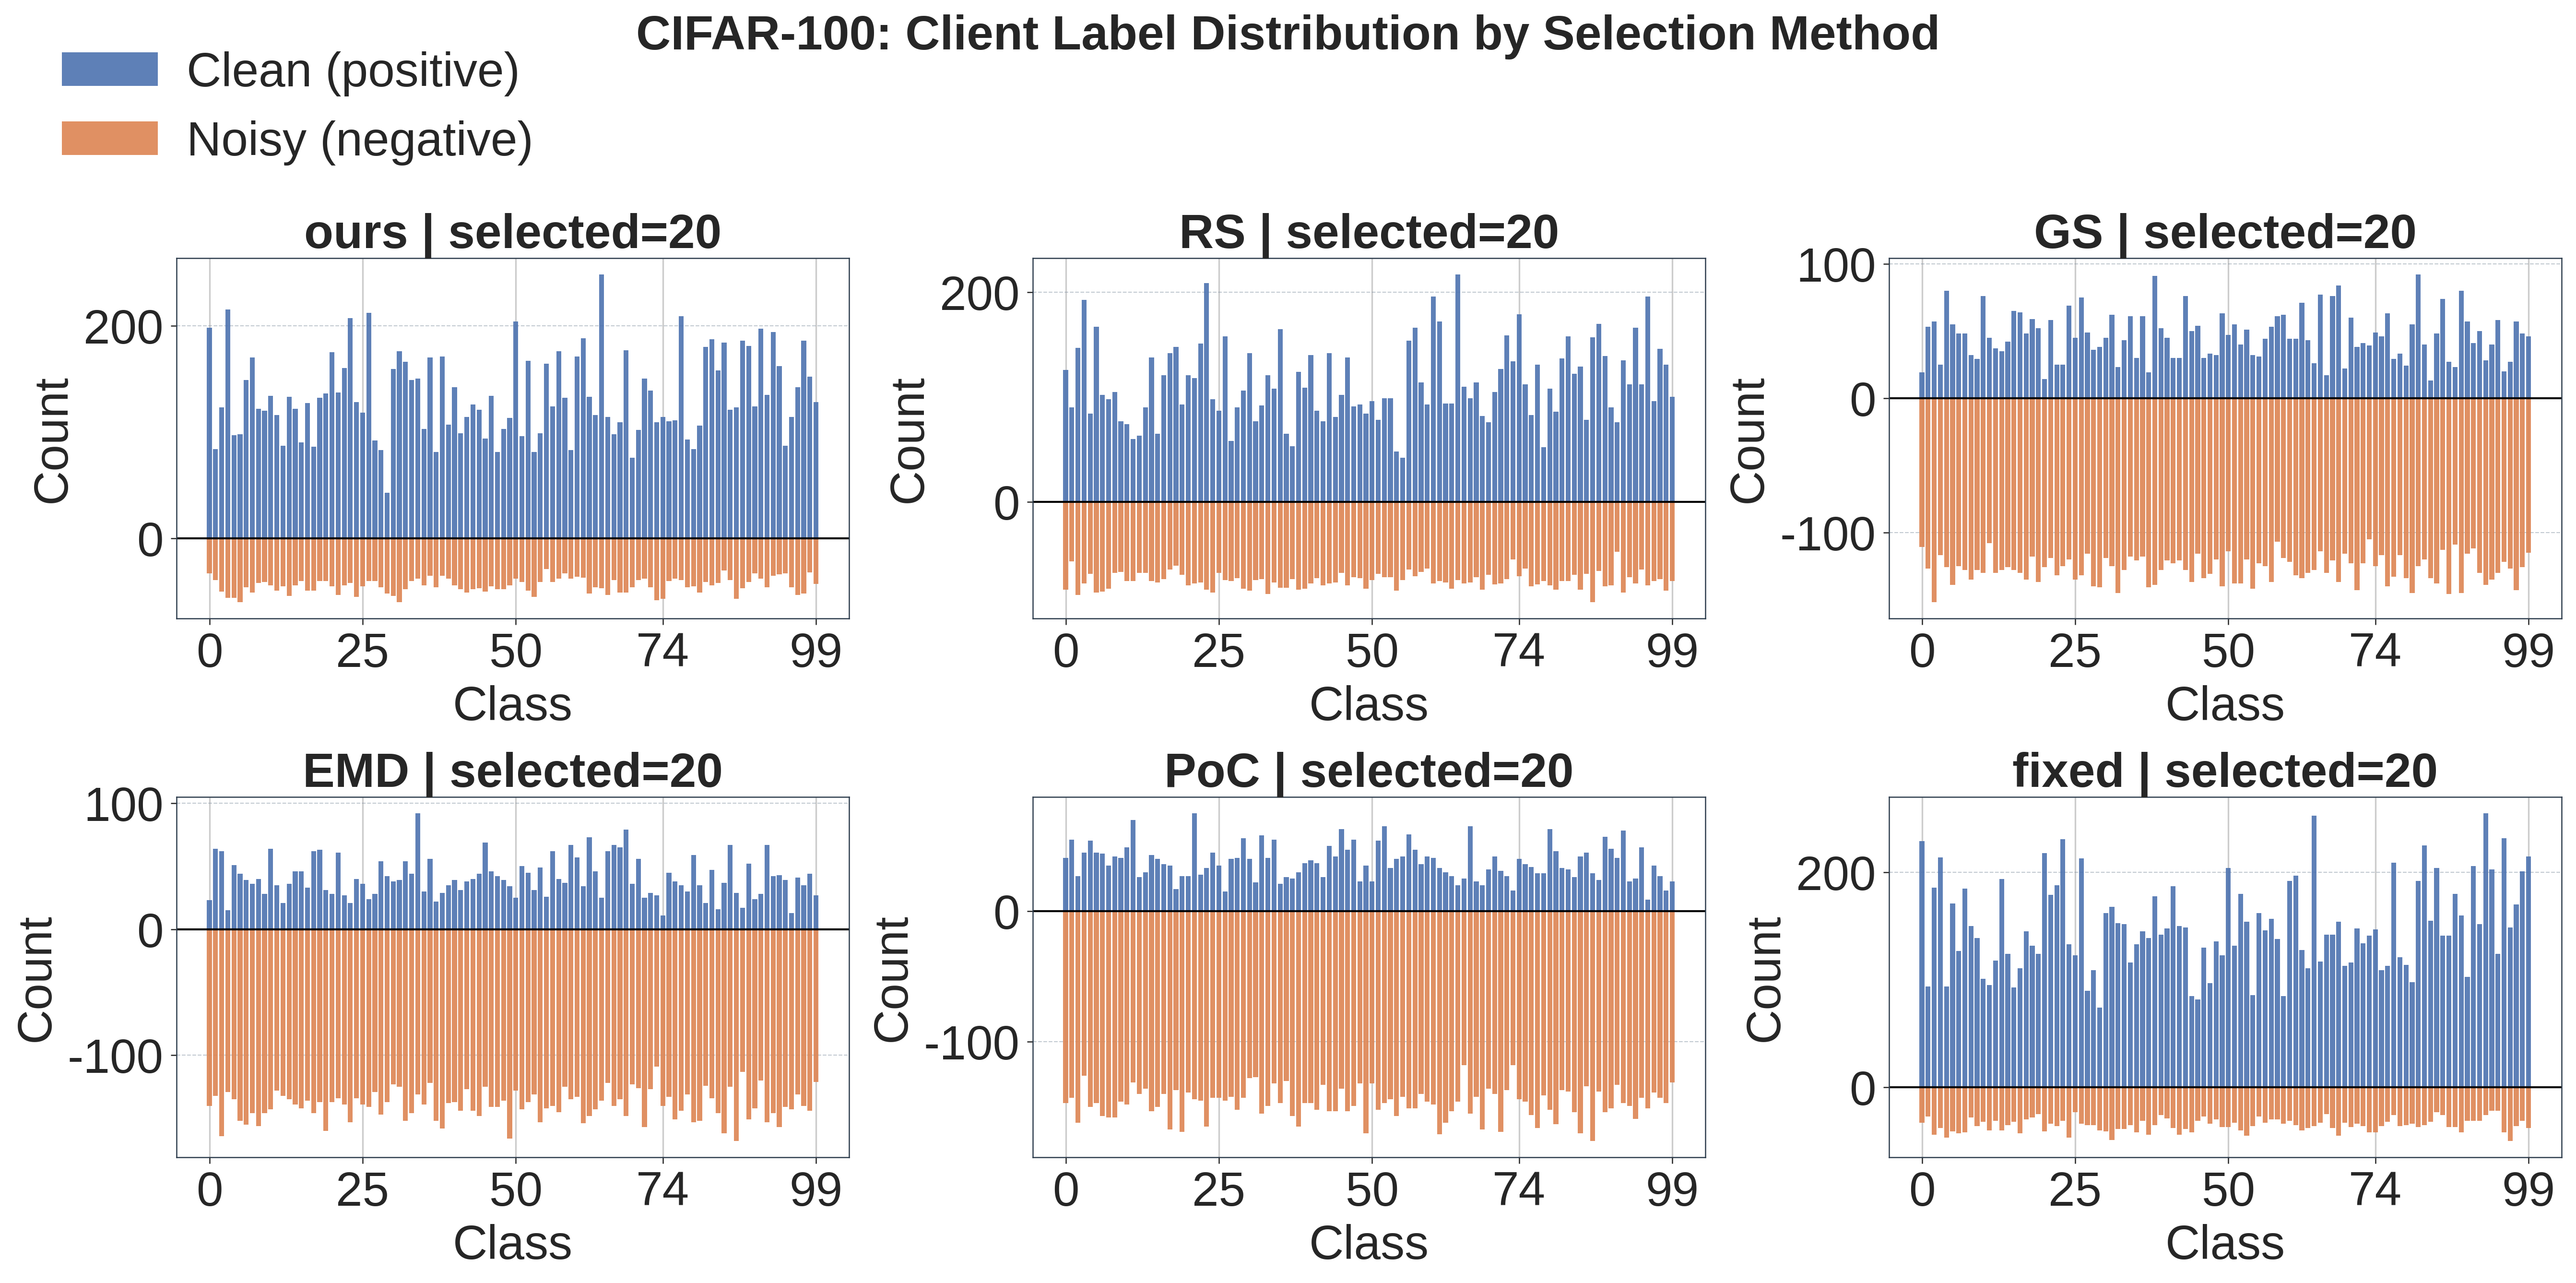
\includegraphics[width=0.48\textwidth]{figure/appendix_subset_cifar100.png}
    \caption{Additional class-wise clean/noisy sample composition of outlier-removal client sets under linear heterogeneous noise. Positive bars denote clean samples, while negative bars denote noisy samples.}
    \label{fig:subset_composition_appendix}
\end{figure}

\section{Additional Client-Scale Experiment}
\label{app:client_scale}

The client-scale experiment complements the main robustness comparisons.
It evaluates whether performance changes monotonically with the number of retained clients.
The resulting curves show that overly small subsets can lose useful class coverage, while overly large subsets can reintroduce noisy or biased clients.
This supports the variable-size outlier-removal design of FedOCR: the goal is not to maximize participation, but to find a retained participant pool that jointly preserves reliability and target-relevant coverage.

\subsection{Greedy retained-budget validation}
\label{app:greedy_budget_validation}
The retained-budget curve below is the appendix version of the greedy-set validation that was summarized in the main text before moving the figure out of the introduction-style discussion.
The curve is non-monotonic: retaining too few clients leaves the pool under-covered, while retaining too many reintroduces accumulated noise.
This is why FedOCR searches for a high-scoring suboptimal retained set rather than maximizing participation blindly.

\begin{figure}[h]
    \centering
    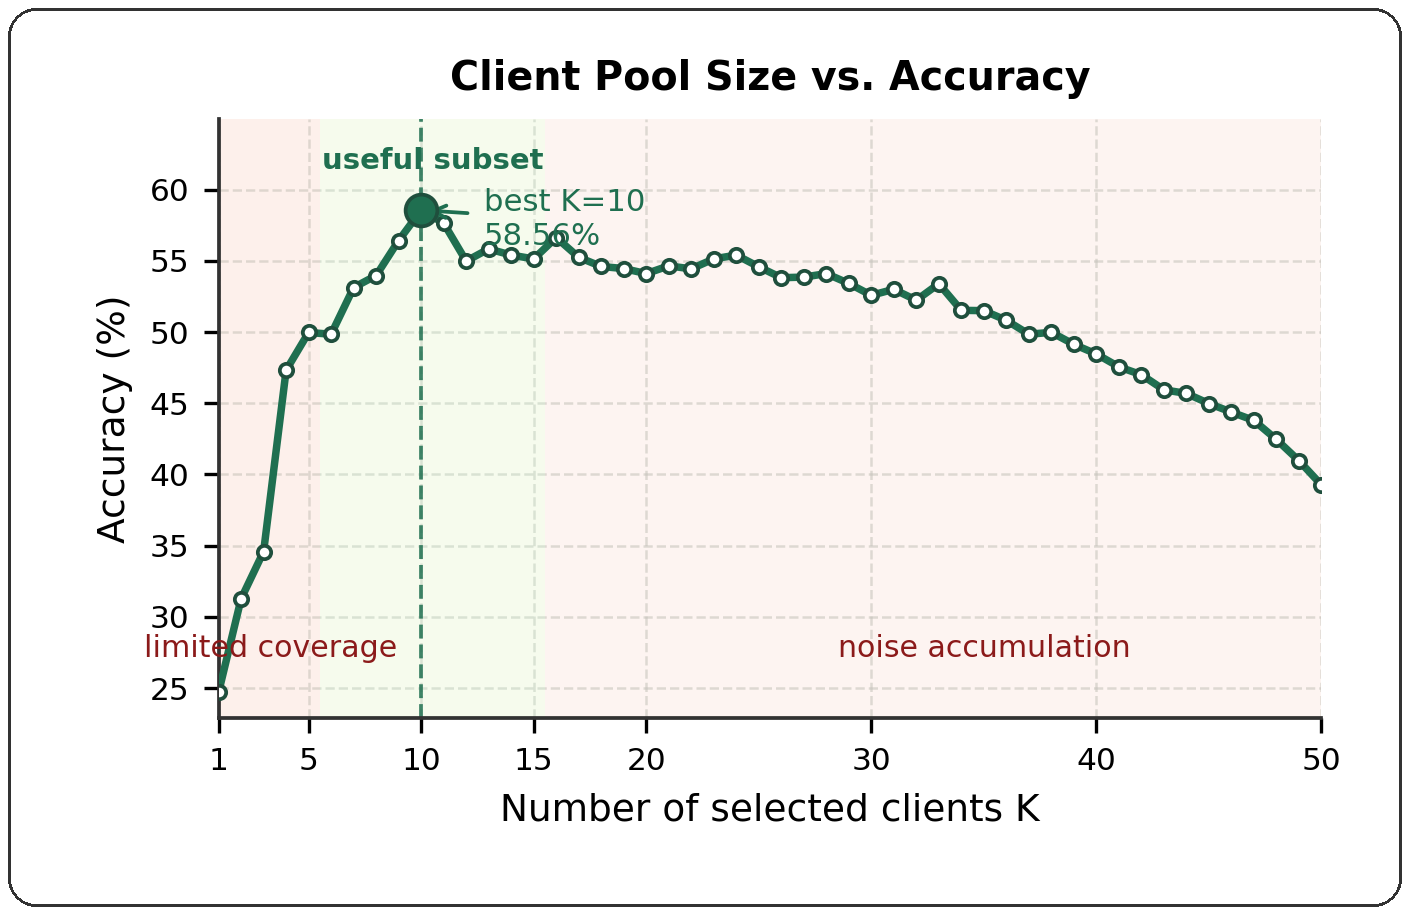
\includegraphics[width=\linewidth]{figure/scale_exp/top50-intro.png}
    \caption{\small Final test accuracy under different retained-client budgets in noisy and Non-IID settings. The curve is non-monotonic: admitting too few clients leaves the retained pool under-covered, while admitting too many reintroduces accumulated noise. This motivates our greedy search for a high-scoring suboptimal retained set rather than a blindly maximal one.}
    \label{fig:greedy_suboptimal}
\end{figure}

\begin{figure*}[h]
    \centering
    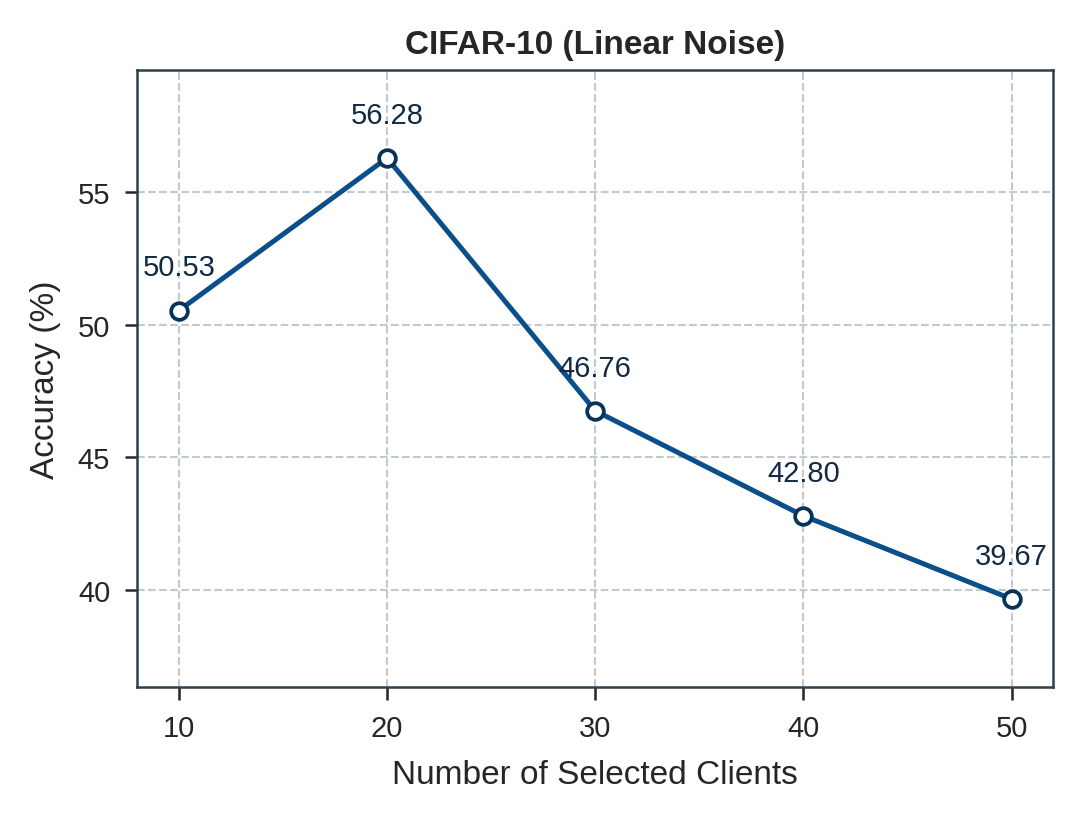
\includegraphics[width=0.31\textwidth]{figure/screening.png}
    \hfill
    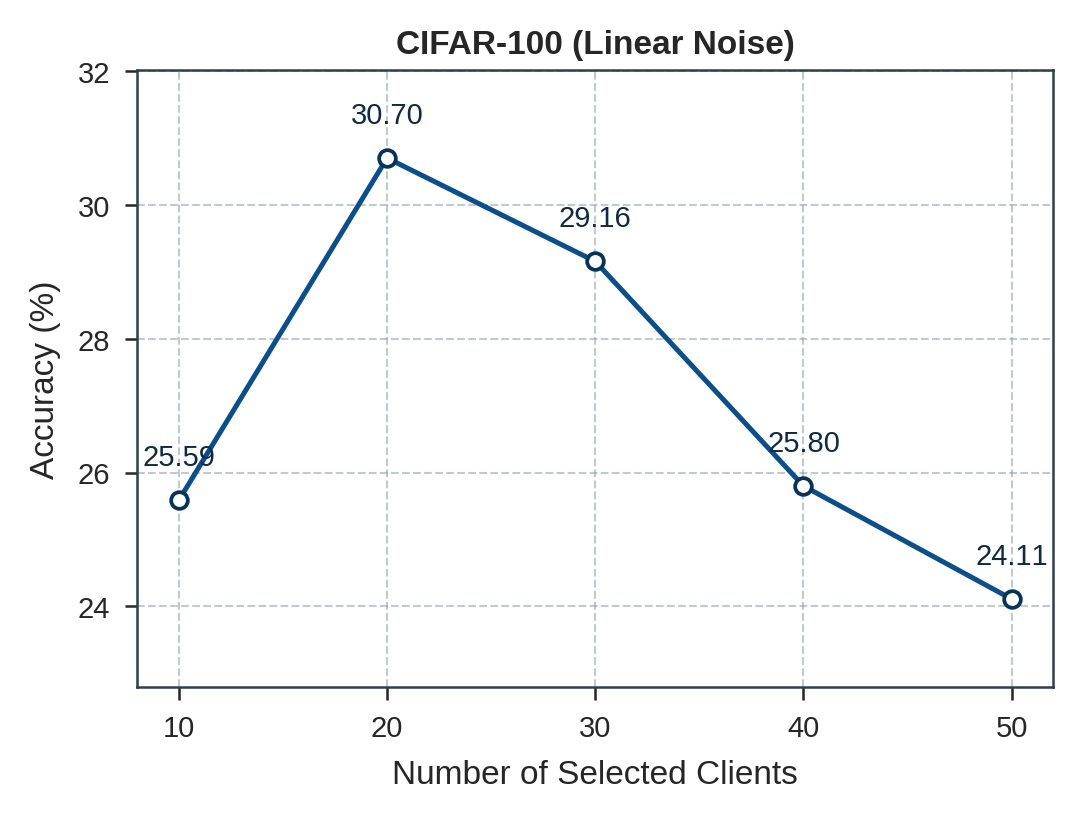
\includegraphics[width=0.31\textwidth]{figure/nips/scale/cifar100.png}
    \hfill
    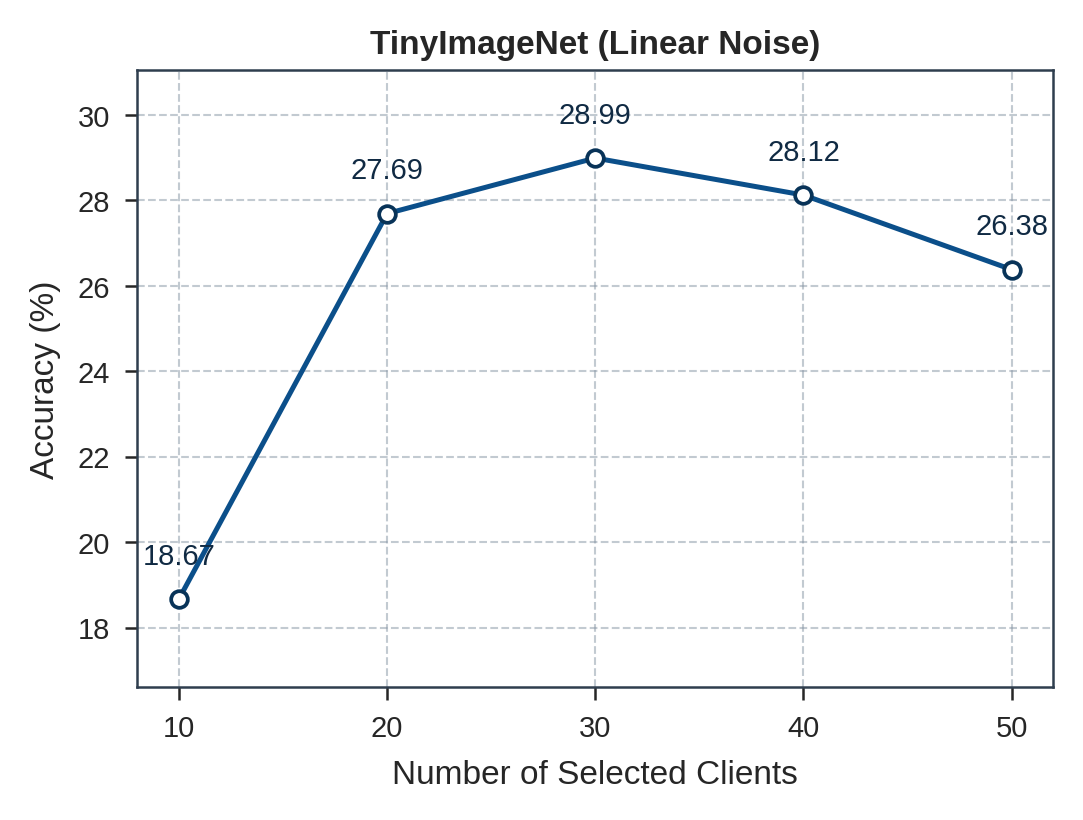
\includegraphics[width=0.31\textwidth]{figure/nips/scale/tinyimagenet.png}
    \caption{Effect of the retained client pool size on final test accuracy under coupled label noise and Non-IID heterogeneity. Performance is non-monotonic with respect to the number of participating clients, showing that retaining an appropriate outlier-removal subset can outperform full participation.}
    \label{fig:screening}
\end{figure*}

\section{Additional Tables and Compatibility Results}
\label{app:additional_results}

\subsection{CIFAR-100 Non-IID Robustness}

Table~\ref{tab:cifar100_noniid_appendix} reports the CIFAR-100 counterpart of the Non-IID robustness experiment under linear heterogeneous noise.
Compared with the CIFAR-10 results in the main text, CIFAR-100 is more challenging and produces lower absolute accuracy.
FedOCR consistently improves over full participation by $3.28$--$4.62$ percentage points and remains competitive across all three heterogeneity levels, while FedNoRo achieves the strongest final accuracy in this full-round comparison.
This result complements the main-table conclusion: the benefit of pre-training client-block outlier removal is visible beyond CIFAR-10, but the relative ranking can change with the dataset difficulty and heterogeneity level.

\begin{table}[h]
\centering
\caption{\normalfont CIFAR-100 accuracy (\%) under linear noise with different Dirichlet Non-IID levels. Results are reported as mean$\pm$standard deviation. Best results are highlighted in bold and second-best results are underlined.}
\label{tab:cifar100_noniid_appendix}
\setlength{\tabcolsep}{4pt}
\renewcommand{\arraystretch}{1.12}
\begin{tabular}{lccc}
\toprule
\textbf{Method} & $\alpha=0.1$ & $\alpha=0.5$ & $\alpha=1.0$ \\
\midrule
All & 18.39$\pm$0.15 & 24.11$\pm$0.15 & 24.17$\pm$0.23 \\
RFA~\cite{pillutla2022robust} & 17.32$\pm$0.17 & 20.52$\pm$0.05 & 21.31$\pm$0.20 \\
FedGreed~\cite{kritharakis2025fedgreed} & 8.73$\pm$1.45 & 20.79$\pm$1.05 & \underline{29.03$\pm$0.85} \\
LASA~\cite{xu2025lasa} & 17.63$\pm$0.11 & 23.69$\pm$0.17 & 25.44$\pm$0.23 \\
FedNed~\cite{lu2024fedned} & 17.57$\pm$0.26 & 23.63$\pm$0.03 & 24.06$\pm$0.20 \\
FedNoRo~\cite{wu2023fednoro} & $\boldsymbol{22.56\pm0.20}$ & $\boldsymbol{30.20\pm0.08}$ & $\boldsymbol{32.82\pm3.79}$ \\
FedCorr~\cite{xu2022fedcorr} & \underline{22.03$\pm$1.01} & 26.19$\pm$0.16 & 24.03$\pm$0.24 \\
FedCS~\cite{hao2025fedcs} & 14.07$\pm$0.26 & 19.84$\pm$0.20 & 21.43$\pm$0.80 \\
FedFixer~\cite{ji2024fedfixer} & 18.66$\pm$0.14 & 23.45$\pm$0.26 & 25.37$\pm$0.23 \\
FedDiv~\cite{li2024feddiv} & 17.73$\pm$0.13 & 22.53$\pm$0.30 & 23.88$\pm$0.21 \\
\midrule
FedOCR (ours) & 21.67$\pm$0.27 & \underline{28.73$\pm$0.72} & 28.93$\pm$0.52 \\
\bottomrule
\end{tabular}
\end{table}
\begin{table}[h]
	\centering
	\caption{\normalfont MedMNIST accuracy (\%) under linear noise with different Dirichlet Non-IID levels. Results use the same best-test-accuracy protocol as Table~\ref{tab:noisy_fl_accuracy} and are reported as mean$\pm$standard deviation. Best results are highlighted in bold and second-best results are underlined.}
	\label{tab:medmnist_noniid_appendix}
	\setlength{\tabcolsep}{5pt}
	\renewcommand{\arraystretch}{1.10}
	\begin{tabular}{lccc}
		\toprule
		\textbf{Method} & $\alpha=0.1$ & $\alpha=0.5$ & $\alpha=1.0$ \\
		\midrule
		All & 46.55$\pm$1.44 & 60.89$\pm$1.89 & 67.68$\pm$1.72 \\
		RFA~\cite{pillutla2022robust} & 38.82$\pm$1.50 & 63.38$\pm$3.24 & 61.60$\pm$1.47 \\
		FedGreed~\cite{kritharakis2025fedgreed} & 21.18$\pm$0.00 & \underline{83.09$\pm$3.17} & $\boldsymbol{89.33\pm2.27}$ \\
		LASA~\cite{xu2025lasa} & 38.97$\pm$0.86 & 54.97$\pm$0.51 & 57.08$\pm$1.91 \\
		FedNed~\cite{lu2024fedned} & 45.50$\pm$2.12 & 64.29$\pm$0.54 & 67.96$\pm$1.49 \\
		FedNoRo~\cite{wu2023fednoro} & 33.92$\pm$2.13 & $\boldsymbol{85.48\pm0.41}$ & 78.07$\pm$0.51 \\
		FedCorr~\cite{xu2022fedcorr} & 4.88$\pm$0.86 & 55.54$\pm$13.10 & 69.09$\pm$9.95 \\
		FedCS~\cite{hao2025fedcs} & 24.66$\pm$1.40 & 56.60$\pm$3.02 & 79.06$\pm$1.39 \\
		FedFixer~\cite{ji2024fedfixer} & \underline{46.72$\pm$1.47} & 61.06$\pm$1.92 & 67.85$\pm$1.75 \\
		FedDiv~\cite{li2024feddiv} & 46.41$\pm$1.46 & 60.75$\pm$1.91 & 67.54$\pm$1.74 \\
		\midrule
		FedOCR (ours) & $\boldsymbol{47.71\pm1.08}$ & 81.05$\pm$0.80 & \underline{86.82$\pm$0.10} \\
		\bottomrule
	\end{tabular}
\end{table}

\subsection{MedMNIST Non-IID Robustness}

Table~\ref{tab:medmnist_noniid_appendix} reports the MedMNIST counterpart of the Non-IID robustness experiment under linear heterogeneous noise.
The results show that the relative ranking is dataset dependent: FedOCR achieves the strongest accuracy at strong Non-IID, while FedNoRo and FedGreed are strongest at moderate and weak Non-IID levels, respectively.
This behavior is consistent with the role of the outlier-removal stage.
When heterogeneity is strong, filtering noisy and target-mismatched clients can provide a clearer benefit because full participation mixes highly incompatible local objectives.
When heterogeneity becomes weaker, the advantage shifts toward methods that exploit more participants during optimization.
Therefore, the MedMNIST appendix result should be read together with the cost analysis in the main text: FedOCR is designed to provide a reliable and efficient retained participant pool, rather than to maximize final accuracy in every single dataset column.


